\documentclass{article}
\usepackage{graphicx}
\usepackage{geometry}
\geometry{a4paper, margin=1in}

\title{Wing Optimization Report}
\date{2025-06-04}

\begin{document}
\maketitle

\section{Executive Summary}
This report summarizes the results of an optimization study conducted to minimize the drag coefficient (CD) of a wing while maintaining a lift coefficient (CL) of 2.0. The wing design was parameterized by taper, twist, and sweep, with constraints on the wing area (S = 100 m²) and span (b = 10 m). The optimization process, utilizing the SLSQP algorithm, exited with a "FAIL" status, indicating that it did not converge successfully.

\section{Problem Formulation}
The optimization problem was formulated as follows:
\begin{itemize}
    \item Objective Function: Minimize drag (CD)
    \item Trim Condition: CL = 2.0
    \item Geometric Constraint: Wing area (S) = 100 m², Span (b) = 10 m
    \item Design Variables: Taper, Twist, Sweep
\end{itemize}

\section{Optimization Setup}
The optimization was performed using the SLSQP algorithm. The optimization ran for 183 iterations and a wall clock time of approximately 3 seconds. The maximum number of iterations was set to 200.

\section{Results and Analysis}
The optimization process concluded with a "FAIL" status, failing to converge to an optimal solution. The final drag coefficient (CD) achieved was 0.1184. The lift distribution is very close to the elliptical lift distribution, suggesting the wing is operating efficiently from an induced drag perspective. However, the twist distribution is constant, which is not typical for an optimized wing and warrants further investigation. As observed in the OpenMDAO Optimization Report for Problem RunOAS, the final values of the optimization loop are shown (See figure 1).

\begin{figure}[h!]
    \centering
    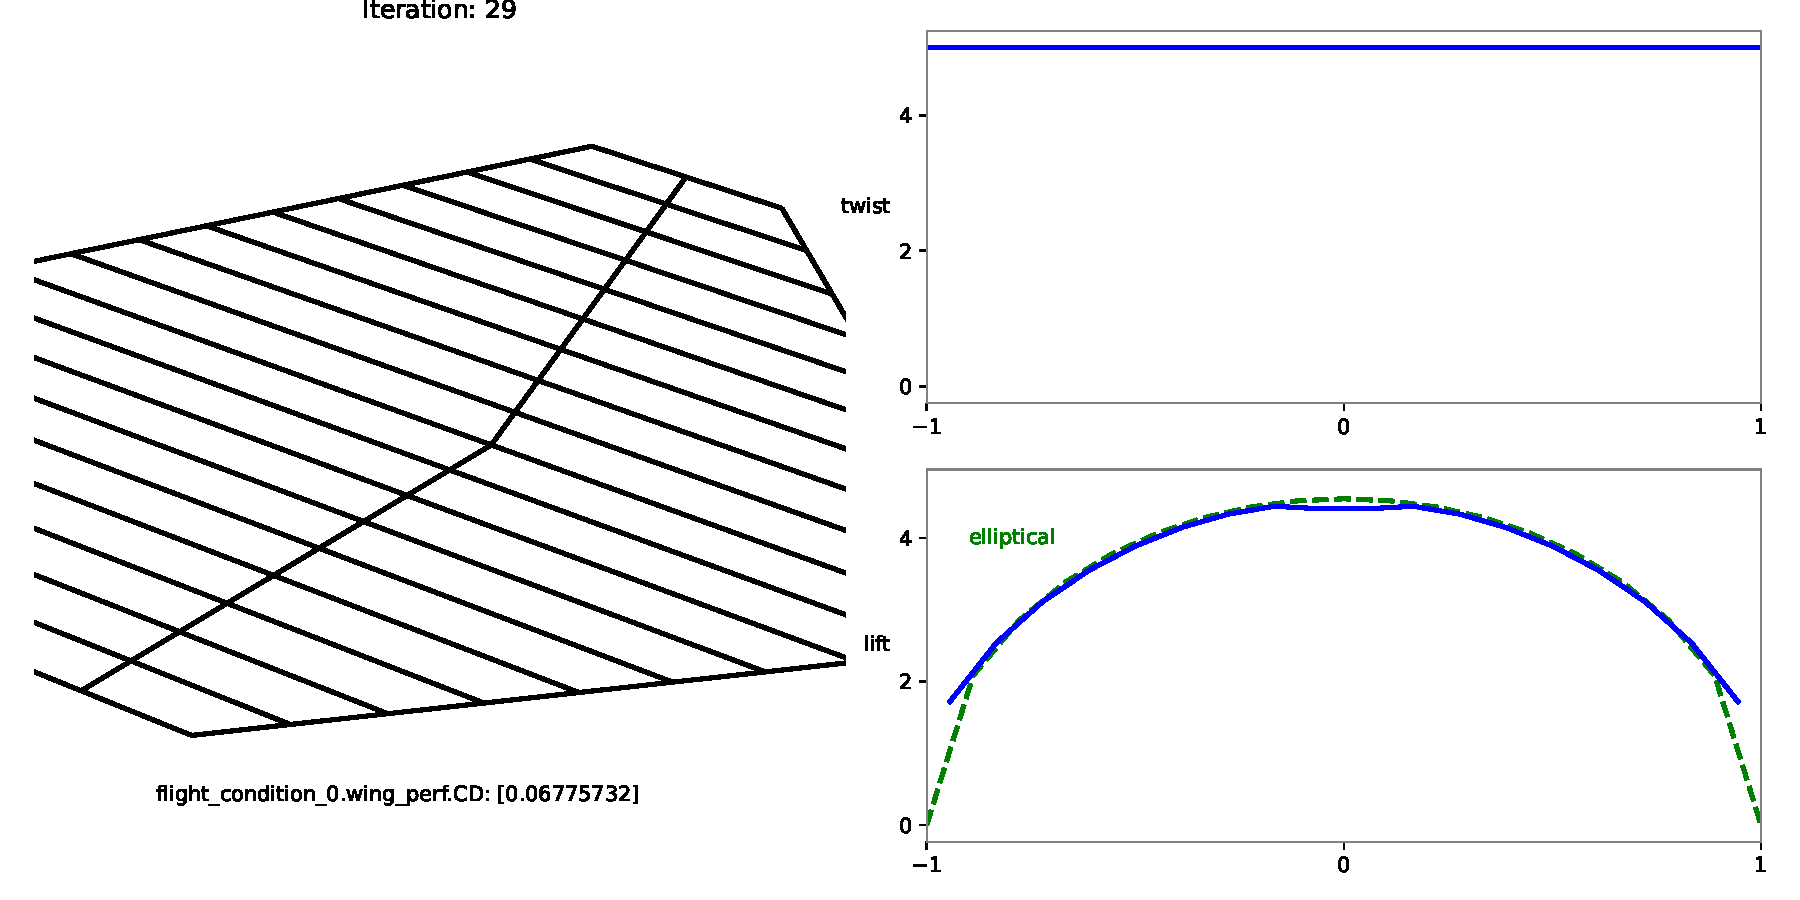
\includegraphics[width=0.75\textwidth]{./Optimized_Wing.pdf}
    \caption{Optimized Visualization of the Wing}
    \label{fig:optimized_wing}
\end{figure}


\section{Recommendations}
Given the optimization's failure to converge, several strategies should be considered:
\begin{itemize}
    \item Examine Design Space: Ensure that the bounds of the design variables (taper, twist, and sweep) are not overly restrictive and that a feasible solution exists within the defined constraints.  It should be noted, however, that the design variables appear to be relatively unconstrained in the optimization report.
    \item Explore Alternative Optimization Algorithms: Since SLSQP struggled to converge, consider using a different optimization algorithm, such as a genetic algorithm, which may be more robust for this particular problem.
    \item Increase Maximum Iterations: The optimization was terminated prematurely with a max iteration number of 200. Increasing this value may improve convergence. Consider reducing the number to decrease simulation time if it appears the optimization will fail regardless.
    \item Constrain Twist Distribution: Given the non-physical twist distribution, it is recommended that this be constrained or penalized in some way to ensure more realistic designs are considered.
\end{itemize}

\section{Conclusion}
The optimization process did not converge successfully, indicating that the SLSQP algorithm may not be well-suited for this problem. Further investigation and adjustments to the optimization setup, including exploring alternative algorithms and constraints, are recommended to achieve a more optimal wing design.

\end{document}